\documentclass{beamer}

\usepackage[hungarian]{babel}
\usepackage{amsmath,amssymb,amsfonts}
\usepackage{cite}
\usepackage{hyperref}
\usepackage{multicol}
\usepackage{ulem}
\usepackage[newfloat]{minted}

\usetheme{Darmstadt}
\usecolortheme{orchid}
\useoutertheme{infolines}

\makeatletter
\setbeamertemplate{footline}
{
  \leavevmode%
  \hbox{%
  \begin{beamercolorbox}[wd=1\paperwidth,ht=2.25ex,dp=1ex,right]{title in head/foot}%
    \usebeamerfont{title in head/foot}
    \insertframenumber{} / \inserttotalframenumber\hspace*{2ex} 
  \end{beamercolorbox}}%
  \vskip0pt%
}
\makeatother

\title{Per-flow virtual queues}
%\subtitle{Programozható hálózatok kiselőadás}

\author{Kámán Rebeka \and Sárközi Gergely}

\date{2024. 05. 13.}

% Feladatleírás, kisEA célja:
% Minden csoport készüljön egy 10-13 perces előadással, melynek felépítése:
% 1) motiváció,
% 2) feladat bemutatása,
% 3) implementációs terv bemutatása és
% 4) ha van már valamilyen eredmény, akkor annak az összefoglalása, bemutatása.
% Mindent röviden, nem kell sok dia!!!

\begin{document}
\frame{\titlepage}

\section{Motiváció}

\begin{frame}{Fizikai sor}
\begin{figure}
    \centering
    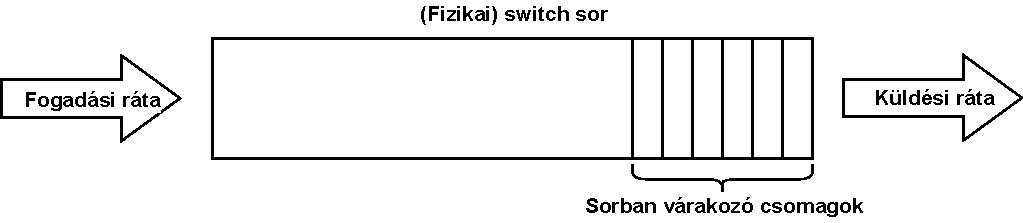
\includegraphics[width=0.9\textwidth]{queue}
\end{figure}
\begin{itemize}
    \item Börsztös forgalom miatt van rá szükség
    \item Egy bizonyos rátával ürül
    \item Megtelik, ha a fogadási ráta tartósan meghaladja a küldési rátát
    \item Egy hosszú sor késleltetést okoz, ezt szeretnénk minimalizálni
\end{itemize}
\end{frame}

\begin{frame}{Virtuális sor}
\begin{itemize}
    \item Emulál egy sort, ami a fizikai sornál kicsit lassabban ürül
    \item A sávszélesség kicsit kevesebb (például $\sim 98\%$)
    \item Nem telítődik meg, nem lesz túl hosszú:
        \begin{itemize}
            \item TCP folyamok $\sim 98\%$-os sávszélességet fogják csak kihasználni
            \item Börsztös forgalom miatt néha pár csomag várakozik
            \item Átlagosan legalább $\sim 2\%$-kal gyorsabban ürül, mint telítődik
        \end{itemize}
\end{itemize}
\end{frame}


\section{Feladat}

\begin{frame}{Feladatleírás}
\begin{itemize}
    \item Minden (aktív) folyam számára egy virtuális sor
        \begin{itemize}
            \item Virtuális és fizikai küldési ráták aránya: $0 < \alpha < 1$
            \item Folyam azonosítás: hasítással vagy táblával
        \end{itemize}
    \item Virtuális sor teli $\implies$ csomag eldobása
    \item Cikk\footnote{https://www.bobbriscoe.net/projects/ipe2eqos/pcn/vq2lb/vq2lb\_tr.pdf}: How to Build a Virtual Queue from Two Leaky Buckets
        \begin{itemize}
            \item Threshold-marking\footnote{https://datatracker.ietf.org/doc/html/rfc5670} alkalmazását ajánlja
            \item Beépített P4 \texttt{meter} megfelelő
            %(simple\_switch, Tofino támogatja, de NetFPGA-SUME állítólag nem)
        \end{itemize}
    \item Cikk\footnote{https://www.bobbriscoe.net/projects/latency/l4saqm\_tr.pdf}: The Native AQM for L4S Traffic
        \begin{itemize}
            \item L4S (Low Latency, Low Loss, Scalable Throughput) AQM fejlesztése
            \item Kimeneti portonként $\sim 98\%$-os virtuális sorokat javasol
        \end{itemize}
    \item Per-flow virtual queue gyakorlatilag per-flow rate limiter?
\end{itemize}
\end{frame}

\section{Implementációs terv és jelenlegi állapot}

\definecolor{aqua}{rgb}{0,1,1}

\begin{frame}[containsverbatim]{Adatsík}
\begin{itemize}
    \item L3 forwarding a kiindulási alap:
\begin{minted}[linenos=false, bgcolor=aqua]{c}
table l3_forward { ... } // Filled by control plane
if (l3_forward.apply().miss) { drop(); return; }
\end{minted}
    
    \item Folyam virtuális sorhoz rendelése:
\begin{minted}[linenos=false, bgcolor=aqua]{c}
hash(meta.flow_id, HashAlgorithm.crc32, 0,
    { /* 5-tuple */ }, (1 << FLOW_ID_T_WIDTH));
meta.vq_id = egress_port ++ meta.flow_id;
\end{minted}

    \item Sor telítettség megállapítása és kezelése:
\begin{minted}[linenos=false, bgcolor=aqua]{c}
meter((1 << VQ_ID_T_WIDTH), MeterType.packets) vq;
vq.execute_meter(meta.vq_id, color);
if (color == METER_YELLOW) { hdr.ipv4.ecn = 0x11; }
else if (color == METER_RED) { drop(); }
\end{minted}
\end{itemize}
\end{frame}

\begin{frame}[containsverbatim]{Vezérlősík}
\begin{itemize}
    \item Python script
    \item L3 forwarding tábla feltöltése \texttt{topology.json} alapján
    \item "Fizikai" és virtuális sor konfigurálása (ráta, méret)
%\begin{verbatim}
%  --queue-rate-pps 500  # 6.0 Mbps
%  --queue-depth-packets 30  # 60.0 ms
%  --vq-committed-alpha 0.2
%  --vq-peak-alpha 0.3
%\end{verbatim}    
    \item Konstans alfa helyett dinamikus alfa érték?
    \begin{itemize}
        \item $\alpha * \text{count}(\text{flows}) > 1 \implies \text{fizikai sor megtelik}$
        \item Folyamok száma \textit{bloom filter}-rel becsülhető
        \item Dinamikus alfa: $\alpha := max(\alpha_\text{min}, \frac{0.98}{\text{count}(\text{flows})})$
        \item Kevés flow esetén sokat javít $\alpha := \alpha_\text{min}$-hez képest
    \end{itemize}
\end{itemize}
\end{frame}

\begin{frame}{Hálózat}
\begin{figure}
    \centering
    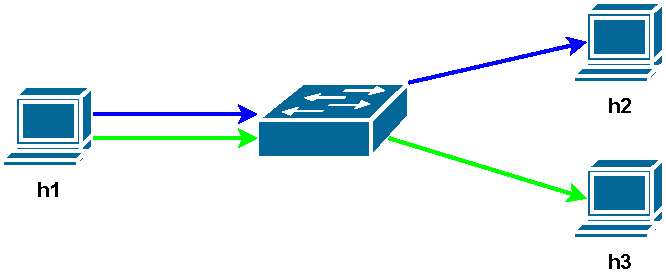
\includegraphics[width=0.6\textwidth]{net}
\end{figure}
\begin{itemize}
    \item L3 címkiosztási stratégia (\texttt{net.l3()})
    \item Vezérlősík automatikus elindítása (\texttt{net.execScript(...)})
    \item Automatikus traffik generálás Mininet task-ok és iperf3 segítségével
        \begin{itemize}
            \item Kis- és nagyobb méretű folyamok vegyesen
            \item Minden folyam adott ideig fut párhuzamosan
        \end{itemize}
    \item Terv: DCTCP használata ECN támogatás érdekében
\end{itemize}
\end{frame}

\begin{frame}{Szimulációs eredmények kiértékelése (terv)}
\begin{itemize}
    \item Adatsíkban log-olunk adatokat: 5-tuple, méret, queue delay, stb.
    \item Különböző grafikonok készítése
    \begin{itemize}
        \item Kicsi és nagy folyamokhoz külön
        \item Átküldött adatmennyiség (boxplot)
        \item Queue delay kumulatív eloszlásfüggvénye
    \end{itemize}
    \item Összehasonlítás:
    \begin{itemize}
        \item Különböző $\alpha$ értékek
        \item Virtuális sor folyamonként
        \item Virtuális sor portonként
        \item Virtuális sor nélkül
    \end{itemize}
\end{itemize}
\end{frame}

\end{document}
